\chapter{共形映射与开弦散射规定}

\lectureoverview{共形映射最初是作为二维静电学的一种实用对称性而出现的。复可微性把这种对称性变成了一种可计算的对称性：柯西--黎曼方程蕴含拉普拉斯方程，而与方向无关的复导数保持角度不变。有了这套工具，弦的世界面就可以画成条带、半平面、圆柱或圆盘，而物理不变。开弦散射于是变成圆盘上的高斯路径积分，动量插入位于其边界上，随后再对它们的不等价位置进行积分。}

\section{二维世界中的静电学}

我们从一个字面意义上的二维静电学问题开始。电荷及其场线被限制在一个平面内；它们并不只是运动恰好发生在平面内的普通三维电荷。于是高斯定律给出
\begin{equation}
  F(r)\propto \frac{1}{r},
  \qquad
  V(r)\propto \log r,
  \label{eq:l08-two-dimensional-coulomb}
\end{equation}
因为通量穿过的是一个周长按\(r\)增长的圆。

用标量势\(\phi\)来表示场。按照黑板上使用的符号约定，
\begin{equation}
  \mathbf E=\nabla\phi,
  \qquad
  \nabla\cdot\mathbf E=\rho,
\end{equation}
因此
\begin{equation}
  \nabla^2\phi
  =\frac{\partial^2\phi}{\partial x^2}
  +\frac{\partial^2\phi}{\partial y^2}
  =\rho.
  \label{eq:l08-poisson}
\end{equation}
在无电荷区域，这化为拉普拉斯方程，
\begin{equation}
  \nabla^2\phi=0.
  \label{eq:l08-laplace-phi}
\end{equation}
\editorialnote{许多电动力学教材定义
\(\mathbf E=-\nabla\Phi\)，在这种情况下，吸收常数后得到
\(\nabla^2\Phi=-\rho\)。本讲使用相反的势符号。无源方程以及所有共形论证都不变。}

\begin{figure}[H]
  \centering
  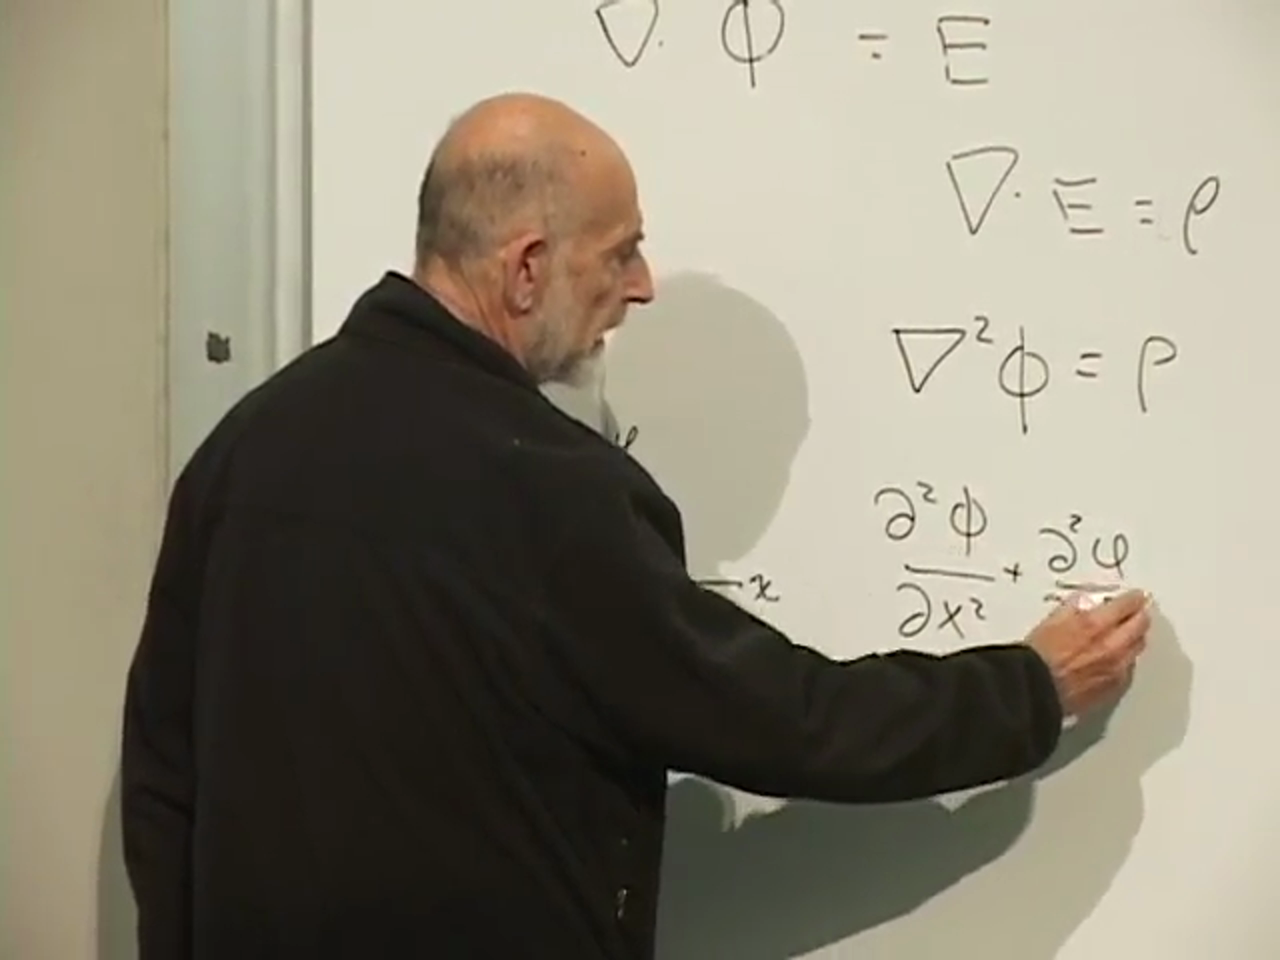
\includegraphics[width=0.72\textwidth]{lecture_08_figure_01.png}
  \caption{静电学方程展开为二维泊松算子。}
  \lectureframe{00:03:48}
  \label{fig:l08-electrostatics-board}
\end{figure}

两个空间导数之间的正号很重要。它使这个方程成为椭圆型方程，而不是波动方程。共形变换保持其无源形式，因此一个区域上的解可以连同其边界条件一起被搬到形状不同的区域上。这在静电学、二维流体流动和制图学中很有用，然后才在弦理论中有用。

\begin{classroomqa}
\audiencequestion{如果拉普拉斯算子为零，这是驻波方程吗？\lecturetimestamp{00:05:35}}
\lecturerresponse{不是。两个空间导数符号相同，而且没有时间导数。波动方程需要时间依赖，并具有洛伦兹式的相对符号。静电学之所以是静态的，正是因为没有任何东西在演化，包括波。}
\end{classroomqa}

\begin{classroomqa}
\audiencequestion{二维中有旋度吗？
\lecturetimestamp{00:06:06}}
\lecturerresponse{有，但它只有一个独立分量。对于
\(\mathbf E=(E_x,E_y)\)，
\[
  \operatorname{curl}_{2d}\mathbf E
  =\partial_yE_x-\partial_xE_y.
\]
可以把它想象为垂直于黑板的分量，尽管一个内禀二维的世界并不需要外部的垂直方向。在更高维中，相应的对象自然是一个反对称二形式。}
\end{classroomqa}

\section{没有优先方向的导数}

在原平面和像平面上引入复坐标：
\begin{equation}
  z=x+iy,
  \qquad
  w=u+iv,
  \qquad
  w=w(z).
  \label{eq:l08-complex-coordinates}
\end{equation}
这里\(x,y,u,v\)是实数。局部地，导数应当是
\begin{equation}
  \frac{dw}{dz}
  =\lim_{\Delta z\to0}\frac{\Delta w}{\Delta z}.
  \label{eq:l08-complex-derivative}
\end{equation}
与实直线不同，复平面允许无穷多个逼近方向。一个连续且通常光滑的映射不必沿每个方向给出相同的比值。

比较两种简单的逼近方式。沿\(x\)方向，\(dy=0\)，所以
\begin{equation}
  \left.\frac{dw}{dz}\right|_x
  =\frac{\partial u}{\partial x}
  +i\frac{\partial v}{\partial x}.
\end{equation}
沿\(y\)方向，\(dx=0\)，并且
\begin{equation}
  \left.\frac{dw}{dz}\right|_y
  =\frac{1}{i}\frac{\partial u}{\partial y}
  +\frac{\partial v}{\partial y}
  =\frac{\partial v}{\partial y}
  -i\frac{\partial u}{\partial y}.
\end{equation}
实部与虚部分别相等给出
\begin{equation}
  \boxed{
  \frac{\partial u}{\partial x}
  =\frac{\partial v}{\partial y},
  \qquad
  \frac{\partial u}{\partial y}
  =-\frac{\partial v}{\partial x}}
  \label{eq:l08-cauchy-riemann}
\end{equation}
这就是柯西--黎曼方程。在通常的可微性假设下，它们也足以使极限
\eqref{eq:l08-complex-derivative}与方向无关。具有这一性质的函数在该点解析，或称全纯。

\begin{figure}[H]
  \centering
  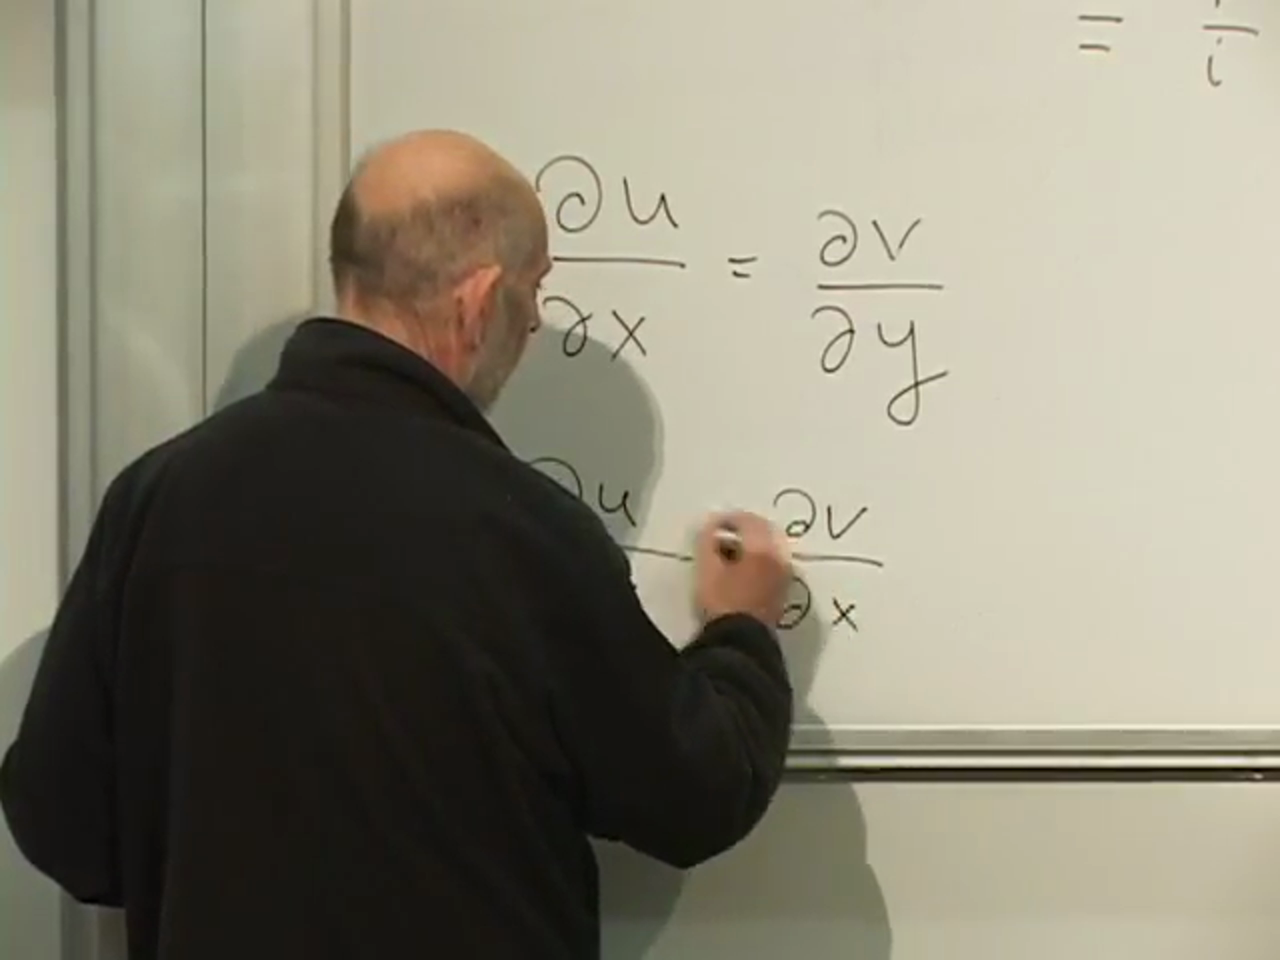
\includegraphics[width=0.70\textwidth]{lecture_08_figure_02.png}
  \caption{完整的柯西--黎曼方程组，包括相对负号。}
  \lectureframe{00:19:48}
  \label{fig:l08-cr-board}
\end{figure}

本讲简要区分了相关术语。在整个有限复平面上全纯的函数称为整函数。亚纯函数可以有孤立极点。因此\(1/z\)在\(z=0\)之外解析，但它不是整函数。

\section{调和共轭与共形几何}

柯西--黎曼方程是一阶耦合方程，但它们蕴含独立的二阶方程。将\(\partial_xu=\partial_yv\)对\(x\)求导，将\(\partial_yu=-\partial_xv\)对\(y\)求导，然后相加：
\begin{align}
  \partial_x^2u&=\partial_x\partial_yv,\\
  \partial_y^2u&=-\partial_y\partial_xv,\\
  \therefore\qquad
  \partial_x^2u+\partial_y^2u&=0.
  \label{eq:l08-harmonic-u}
\end{align}
交换\(u\)与\(v\)重复上述论证，得到
\begin{equation}
  \partial_x^2v+\partial_y^2v=0.
  \label{eq:l08-harmonic-v}
\end{equation}
因此，解析函数的实部和虚部是调和共轭的。两个任意的调和函数并不会自动构成解析函数；它们仍必须由\eqref{eq:l08-cauchy-riemann}相联系。

\begin{figure}[H]
  \centering
  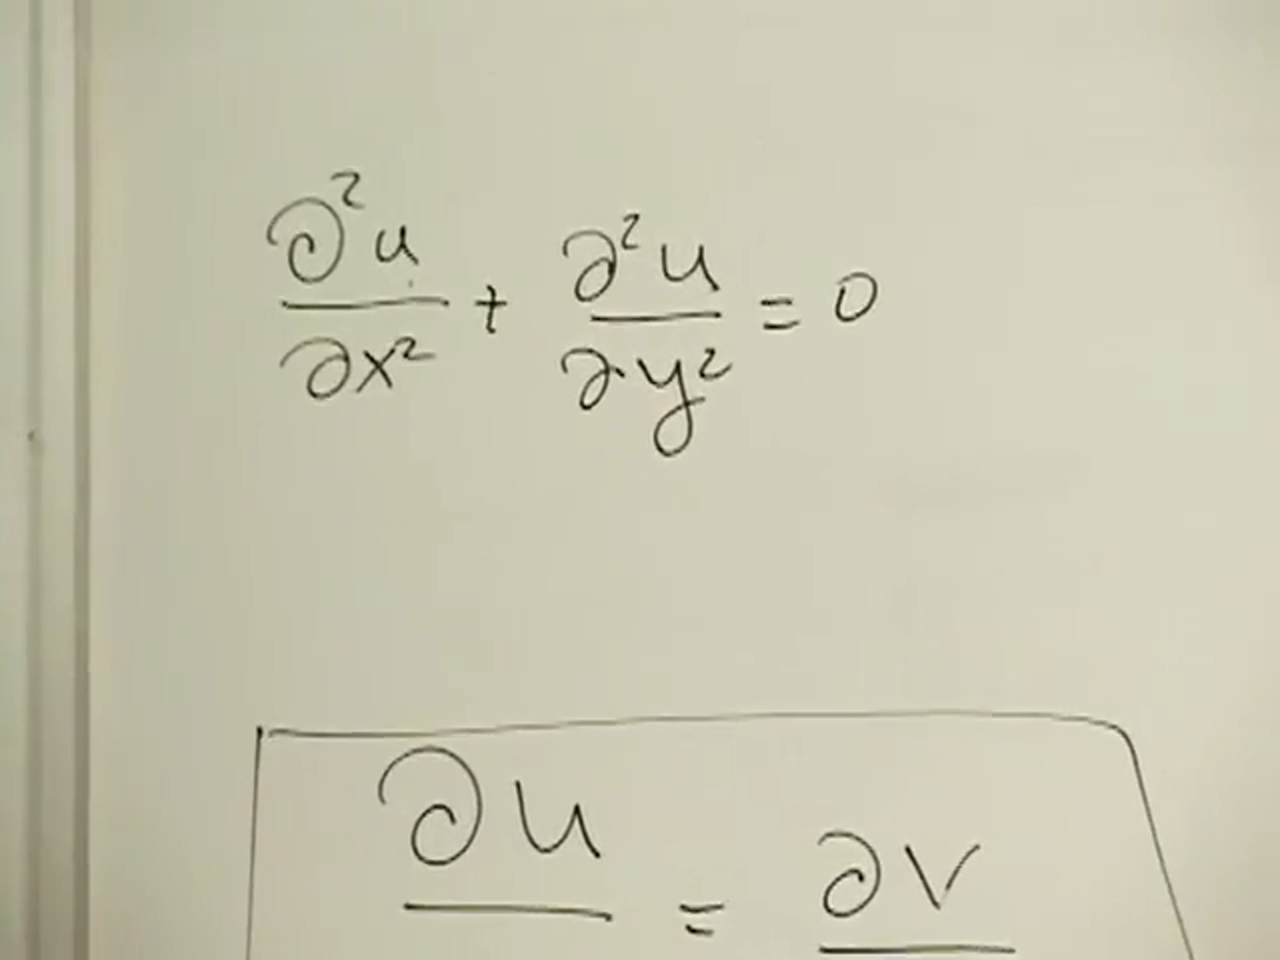
\includegraphics[width=0.68\textwidth]{lecture_08_figure_03.png}
  \caption{混合导数相消，留下解析映射的一个分量所满足的拉普拉斯方程。}
  \lectureframe{00:23:09}
  \label{fig:l08-harmonic-board}
\end{figure}

还有一种有用的矢量解释。若\(\mathbf F=(u,-v)\)，则两个柯西--黎曼方程表明，在所选定向约定下，\(\mathbf F\)的散度和二维旋度均为零。这就是所承诺的回到静电学。

\subsection{为何角度得以保持}

将两个小复位移写成极坐标形式：
\begin{equation}
  \delta z=\rho e^{i\theta},
  \qquad
  \Delta z=\rho'e^{i\theta'}.
\end{equation}
它们的比值具有相位\(\theta-\theta'\)，恰为二者之间的夹角。在解析映射下，
\begin{equation}
  \frac{\delta w}{\delta z}
  =\frac{\Delta w}{\Delta z}
  =w'(z),
\end{equation}
因为导数不依赖于方向。整理可得
\begin{equation}
  \frac{\Delta z}{\delta z}
  =\frac{\Delta w}{\delta w}.
  \label{eq:l08-angle-ratio}
\end{equation}
两边具有相同的相位，因此原区间之间的夹角等于其像之间的夹角。

\begin{figure}[H]
  \centering
  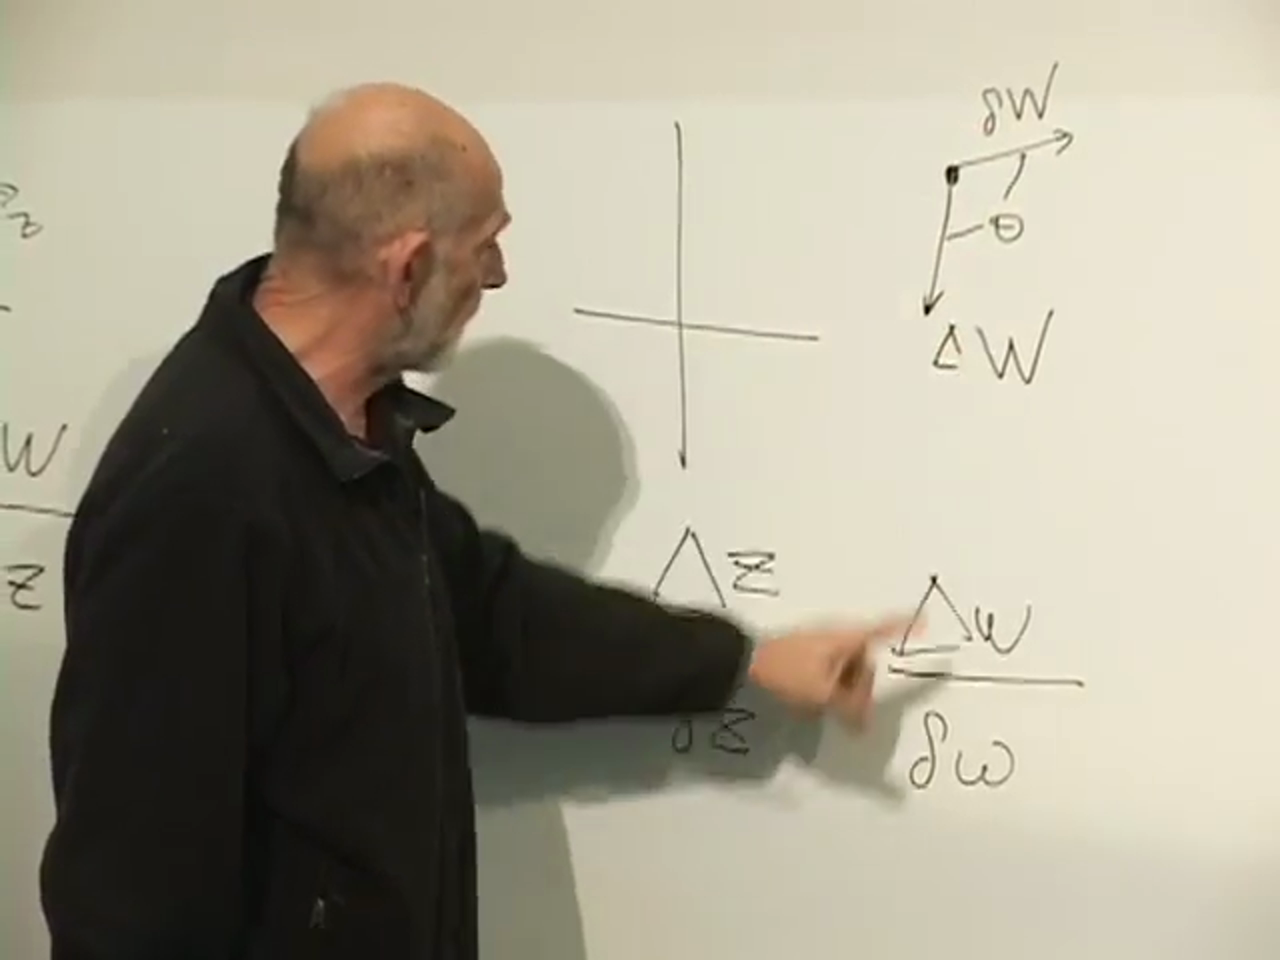
\includegraphics[width=0.70\textwidth]{lecture_08_figure_04.png}
  \medskip

  \begin{tikzpicture}[x=0.9cm,y=0.9cm,>=Latex]
    \begin{scope}
      \draw[->] (-0.2,0) -- (2.3,0);
      \draw[->] (0,-0.2) -- (0,2.1);
      \draw[very thick,blue!65!black,->] (0,0) -- (1.85,0.45)
        node[right] {\(\delta z\)};
      \draw[very thick,orange!75!black,->] (0,0) -- (0.72,1.65)
        node[above] {\(\Delta z\)};
      \draw (0.58,0.14) arc[start angle=14,end angle=66,radius=0.60];
      \node at (1.0,-0.55) {\(z\)-plane};
    \end{scope}
    \draw[->,thick] (3.0,0.9) -- (4.2,0.9)
      node[midway,above] {\(w(z)\)};
    \begin{scope}[xshift=5.0cm]
      \draw[->] (-0.2,0) -- (2.3,0);
      \draw[->] (0,-0.2) -- (0,2.1);
      \draw[very thick,blue!65!black,->] (0,0) -- (1.65,0.70)
        node[right] {\(\delta w\)};
      \draw[very thick,orange!75!black,->] (0,0) -- (0.48,1.62)
        node[above] {\(\Delta w\)};
      \draw (0.54,0.23) arc[start angle=23,end angle=74,radius=0.59];
      \node at (1.0,-0.55) {\(w\)-plane};
    \end{scope}
  \end{tikzpicture}
  \caption{黑板证明与一个清晰的局部重构。乘以\(w'(z)\)会将每个无穷小方向旋转并重新缩放相同的量，从而保持它们的相对角度。}
  \lectureframe{00:34:11}
  \label{fig:l08-angle-proof}
\end{figure}

这一局部论证假设\(w'(z)\neq0\)。在临界点处，映射可能不再是局部一一的，必须单独处理其几何。远离此类点处，解析映射与保向共形映射在局部是同一类对象。

\section{训练眼力的例子}

\subsection{平方映射与复共轭}

对于\(w=z^2\)，
\begin{equation}
  (x+iy)^2=x^2-y^2+2ixy=u+iv,
\end{equation}
因此
\begin{equation}
  u=x^2-y^2,
  \qquad
  v=2xy.
  \label{eq:l08-z-squared-components}
\end{equation}
\(u\)的二阶导数为\(2\)和\(-2\)；\(v\)的二阶导数分别消失。二者都是调和的，直接求导也验证了柯西--黎曼方程。

\begin{figure}[H]
  \centering
  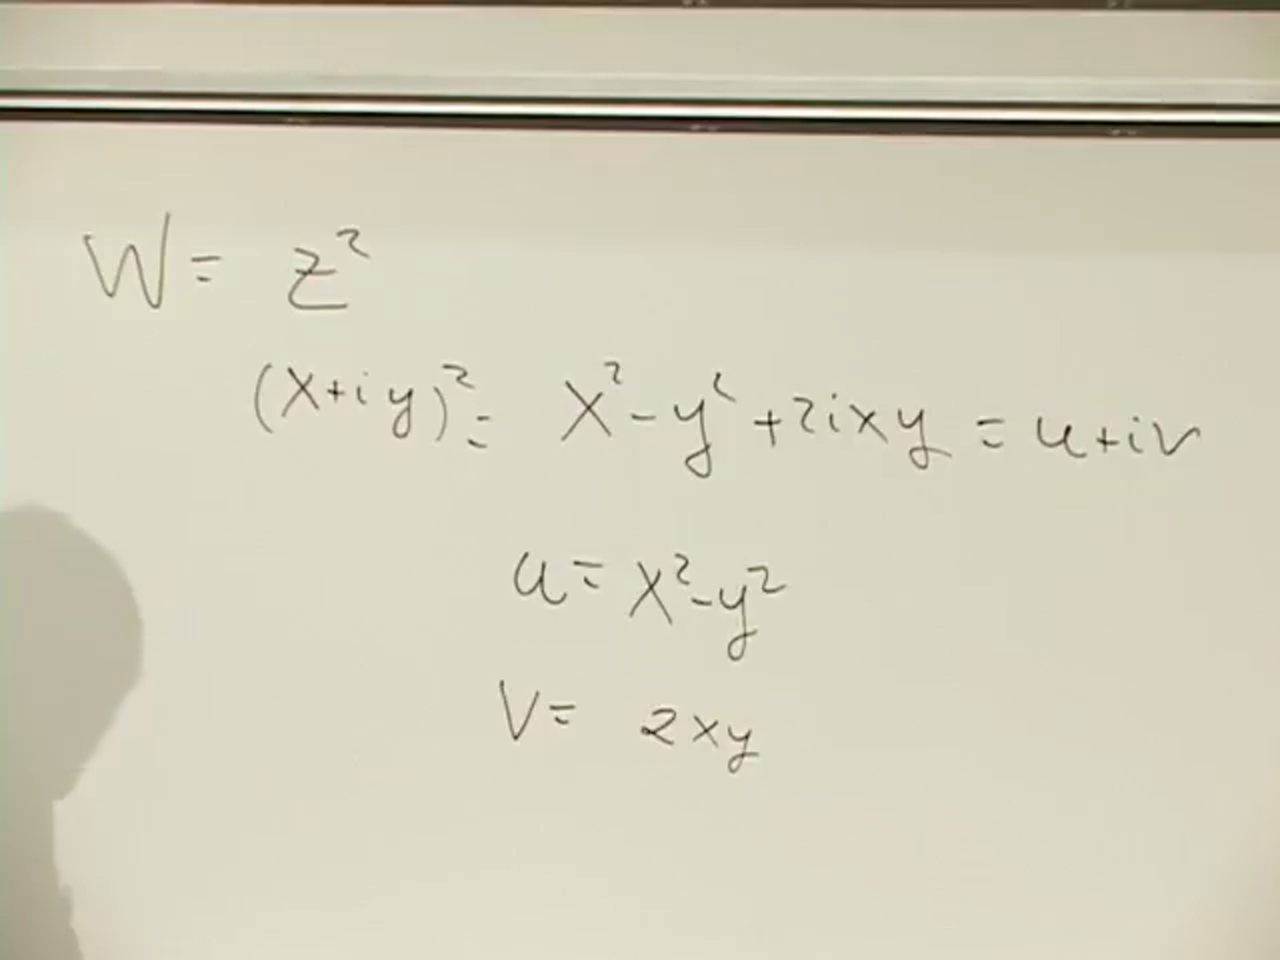
\includegraphics[width=0.72\textwidth]{lecture_08_figure_05.png}
  \caption{平方映射分解为其实部和虚部调和分量。}
  \lectureframe{00:36:45}
  \label{fig:l08-z-square-board}
\end{figure}

\begin{classroomqa}
\audiencequestion{\(1/z\)是否给出一个非解析的例子？
\lecturetimestamp{00:37:49}}
\lecturerresponse{仅在一个点处。它在\(z\neq0\)处解析，并在原点有一个极点。要看到一个处处不满足柯西--黎曼检验的映射，复共轭是更好的例子。}
\end{classroomqa}

相比之下，
\begin{equation}
  w=\bar z=x-iy
  \qquad\Longrightarrow\qquad
  u=x,\quad v=-y
\end{equation}
反转定向。它的导数以符号之差违反第一个柯西--黎曼方程，因此作为\(z\)的函数它不是解析的。

\begin{figure}[H]
  \centering
  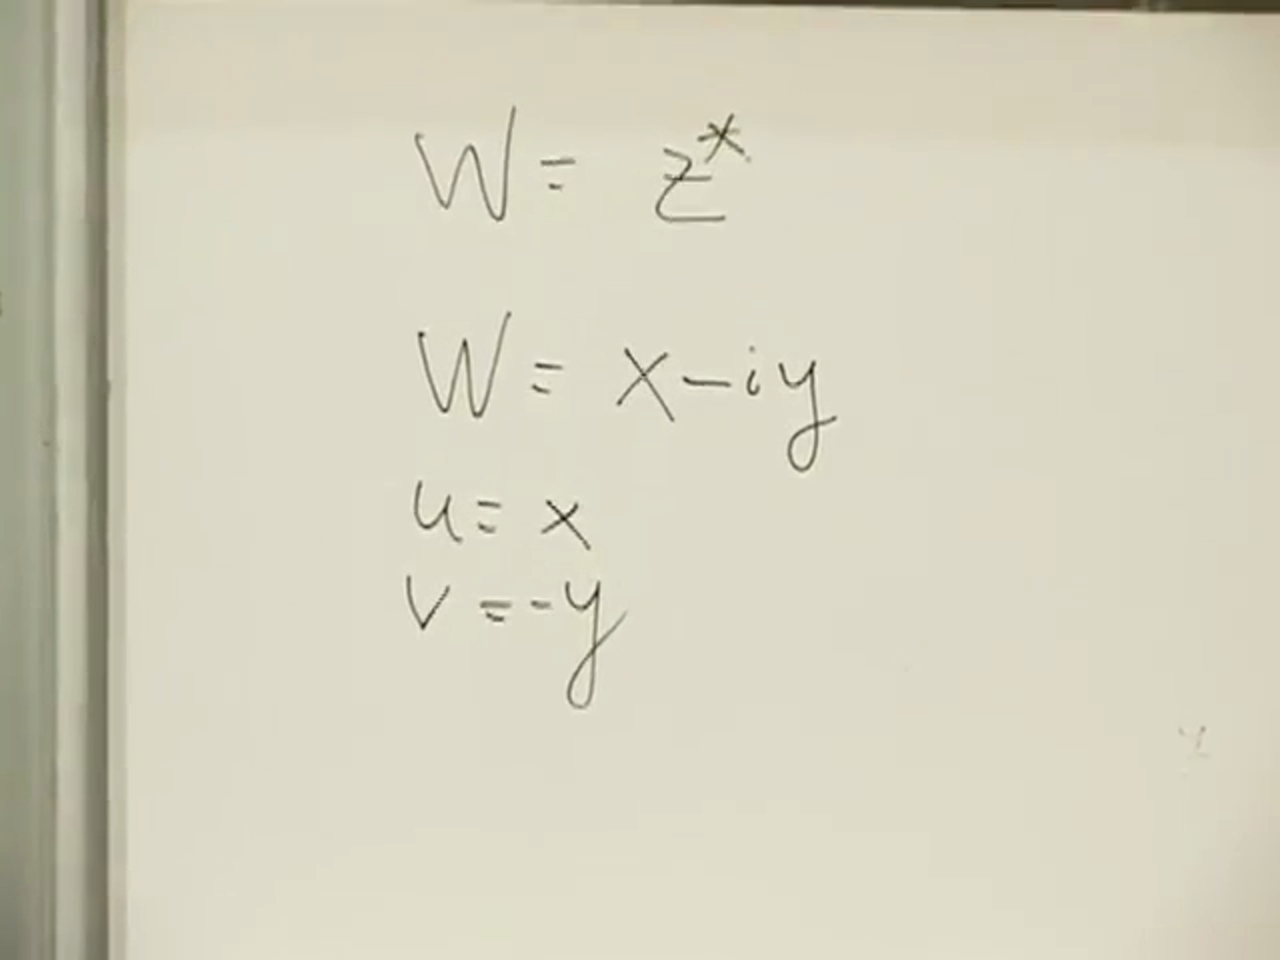
\includegraphics[width=0.62\textwidth]{lecture_08_figure_06.png}
  \caption{复共轭提供了刻意构造的非解析反例。}
  \lectureframe{00:38:38}
  \label{fig:l08-conjugate-board}
\end{figure}

\subsection{指数函数及其反函数}

\begin{classroomqa}
\audiencequestion{若\(e^z\)是解析的，为何其反函数\(\log z\)也应是解析的？\lecturetimestamp{00:40:38}}
\lecturerresponse{在反函数存在且\(w'(z)\neq0\)处，其导数为\(1/w'(z)\)。因此方向无关性得以保持。整体上对数函数是多值的，因此需选择一个分支并排除其分支点和割线。局部共形陈述在该选定区域上仍然成立。}
\end{classroomqa}

欧拉公式给出
\begin{equation}
  w=e^z=e^{x+iy}
  =e^x(\cos y+i\sin y),
\end{equation}
因此
\begin{equation}
  u=e^x\cos y,
  \qquad
  v=e^x\sin y.
  \label{eq:l08-exponential-components}
\end{equation}
例如，\(\partial_xu=e^x\cos y=\partial_yv\)，第二个柯西--黎曼方程同样直接可得。

\begin{figure}[H]
  \centering
  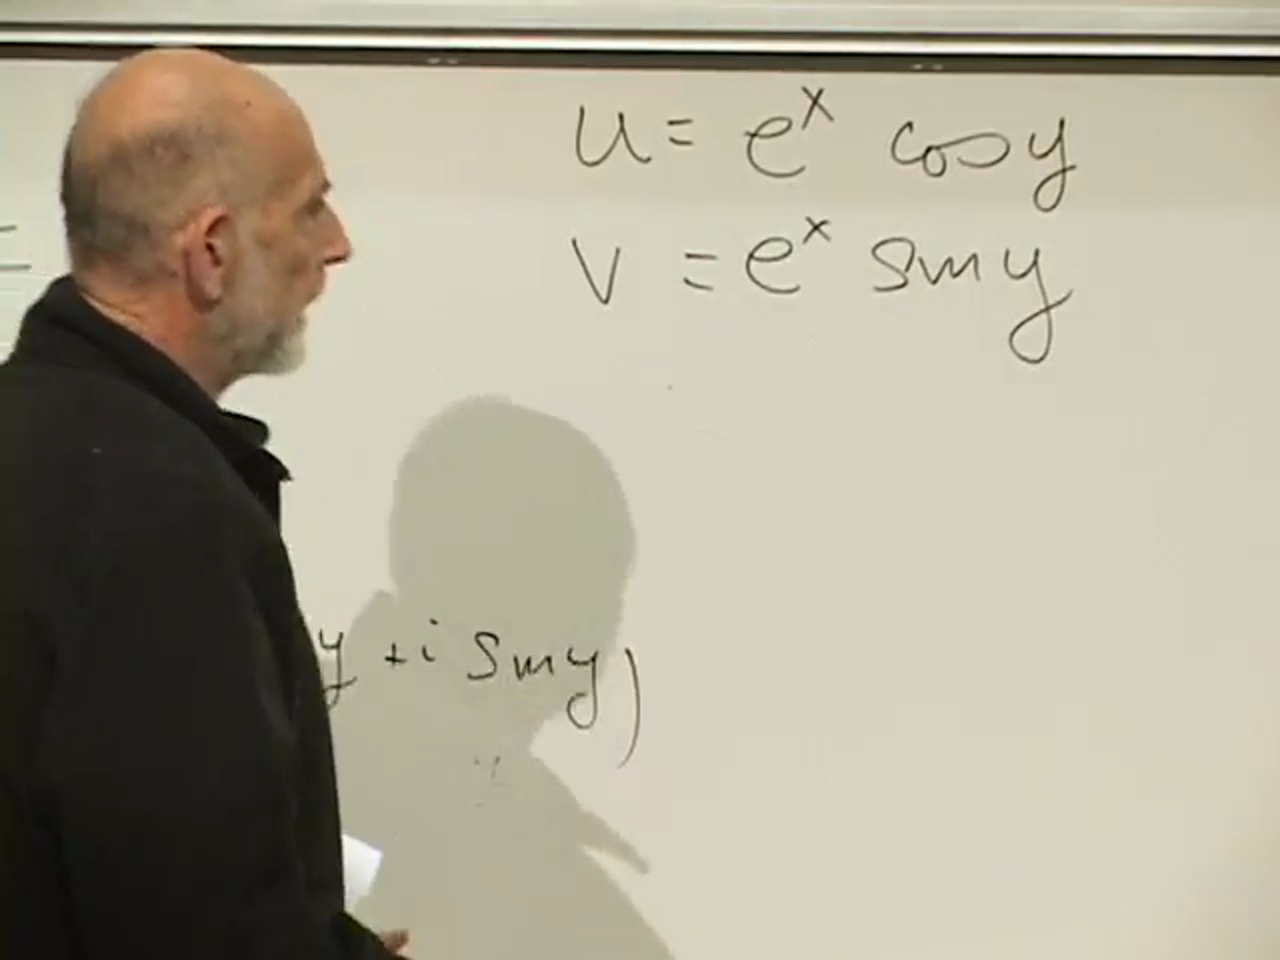
\includegraphics[width=0.68\textwidth]{lecture_08_figure_07.png}
  \caption{指数映射的实部和虚部分量。}
  \lectureframe{00:42:23}
  \label{fig:l08-exponential-board}
\end{figure}

\section{半平面、带形、柱面与圆盘}

\subsection{对数将半径变为时间}

取右半平面，其中\(-\pi/2<\theta<\pi/2\)，并写出
\begin{equation}
  z=re^{i\theta},
  \qquad
  w=\log z=\log r+i\theta.
  \label{eq:l08-log-map}
\end{equation}
该半平面映射到无限带形
\begin{equation}
  -\frac{\pi}{2}<\operatorname{Im}w<\frac{\pi}{2}.
\end{equation}
固定\(\theta\)的射线变为水平线，而固定\(r\)的半圆变为竖直线。原点被送到\(\operatorname{Re}w=-\infty\)，而\(r=\infty\)被送到\(\operatorname{Re}w=+\infty\)。

\begin{figure}[H]
  \centering
  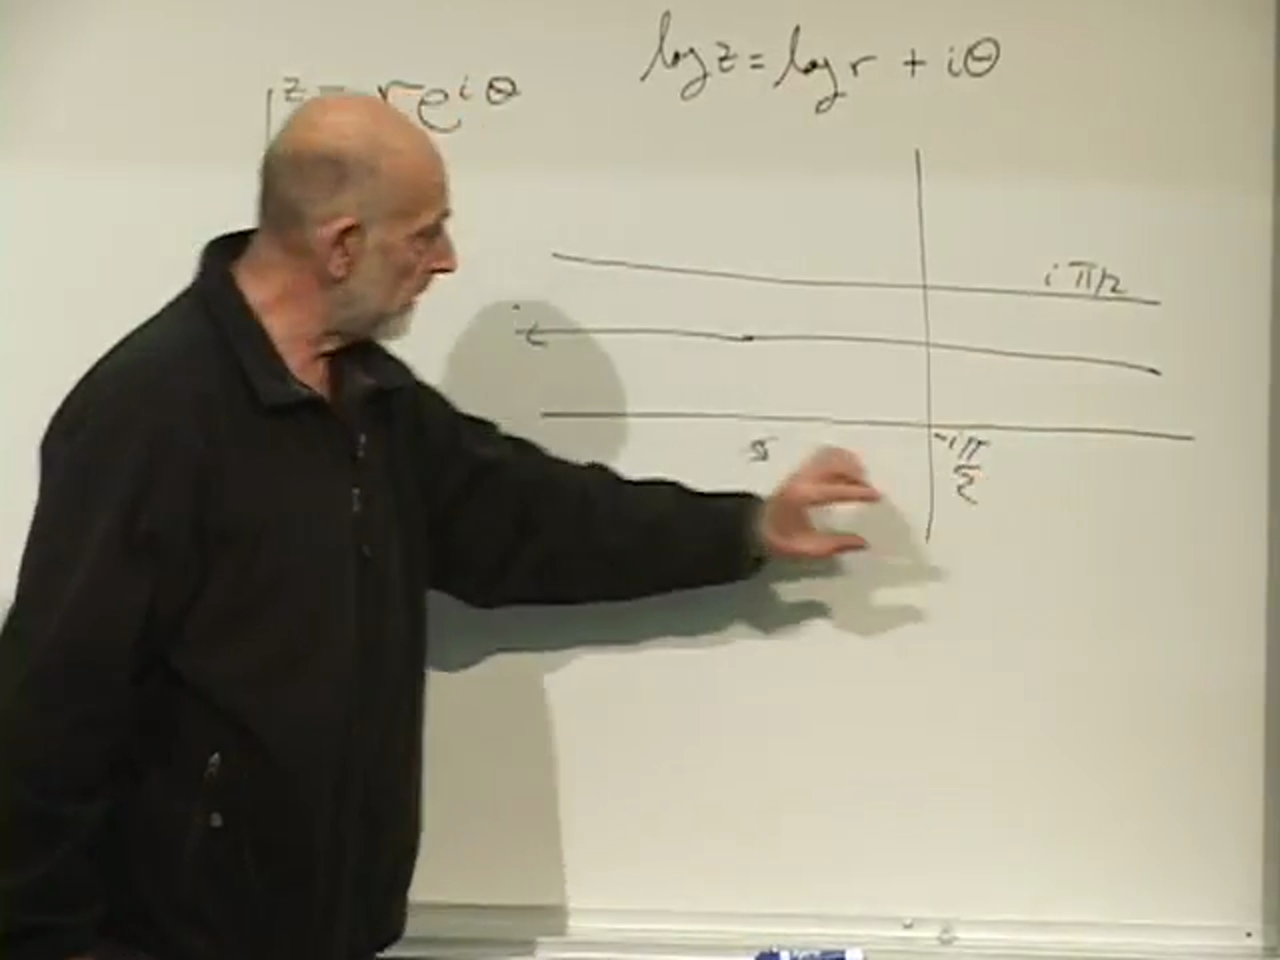
\includegraphics[width=0.75\textwidth]{lecture_08_figure_08.png}
  \caption{对数将右半平面映入一个无限带形：极坐标射线与半圆变为正交的矩形网格。}
  \lectureframe{00:47:48}
  \label{fig:l08-log-strip-board}
\end{figure}

这条带子是开弦的标准世界面。它有界的坐标是沿弦的参数，而沿无界方向的平移则是世界面时间。在逆指数映射下，时间平移变为伸缩\(z\mapsto e^a z\)。因此，同一个对称性在带子上看起来是平移，而在半平面上看起来是均匀膨胀。

\begin{classroomqa}
\audiencequestion{像\(r=1\)这样的特定值会到哪里去，带子上的坐标仍然是极坐标吗？\lecturetimestamp{00:50:58}}
\lecturerresponse{固定半径的圆变成\(\operatorname{Re}w=\log r\)处的竖直线；特别地，\(r=1\)映射到中心线\(\operatorname{Re}w=0\)。极坐标描述\(z\)平面。\(w\)平面使用普通的直角坐标\((\log r,\theta)\)。}
\end{classroomqa}

如果整个去心平面被\(\log z\)映射，则角坐标的周期为\(2\pi\)。因此，所得的带子的上下边缘被等同起来：它是一个无限长圆柱面。带边界的半平面描述开弦世界面；没有边界且角度具有周期性的整个平面描述闭弦圆柱面。

\begin{figure}[H]
  \centering
  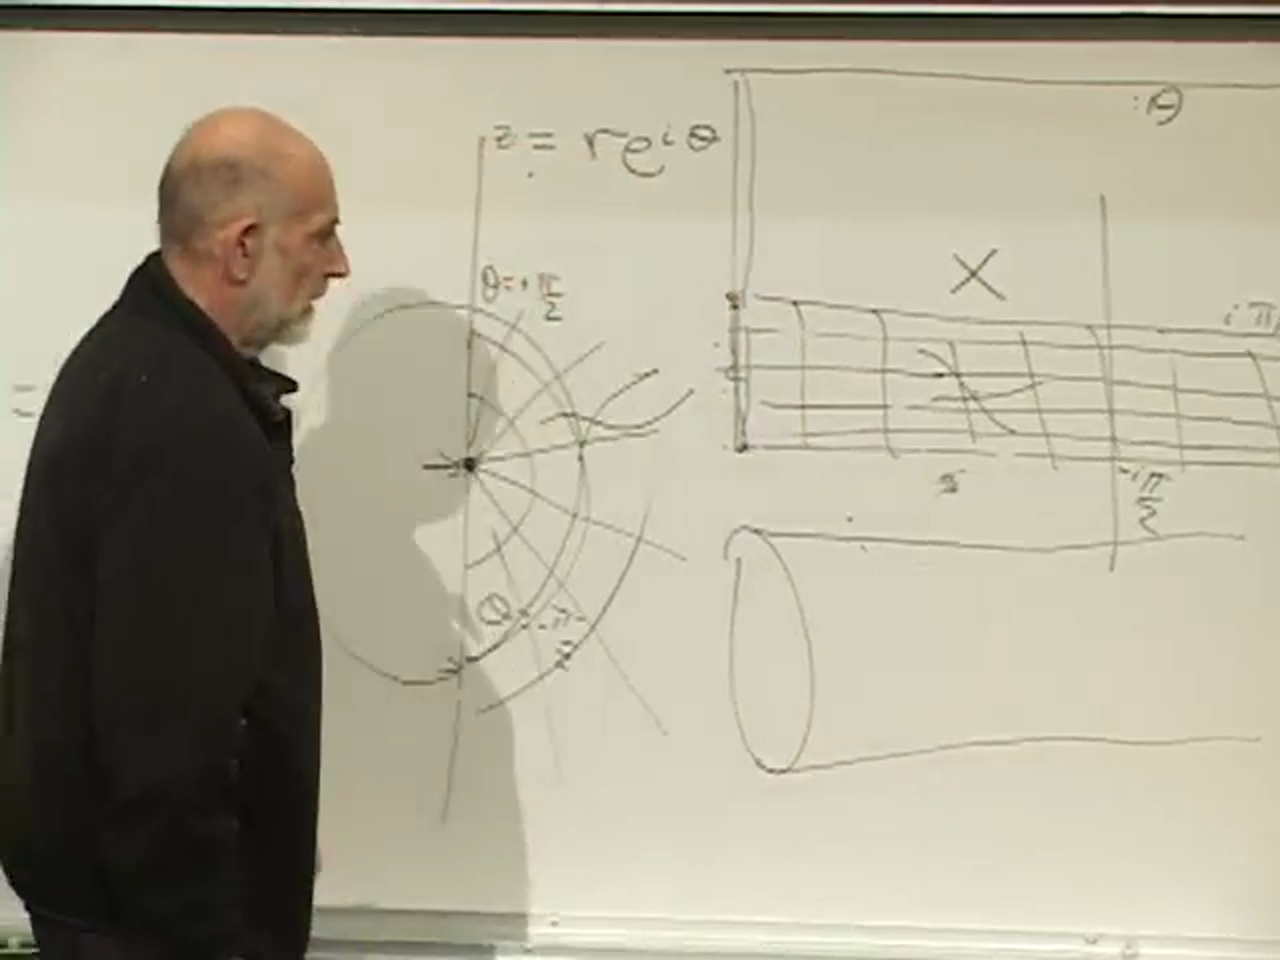
\includegraphics[width=0.75\textwidth]{lecture_08_figure_09.png}
  \caption{半平面/带子图像，以及将整个去心平面变成闭弦圆柱面的周期性等同。}
  \lectureframe{00:54:23}
  \label{fig:l08-open-closed-board}
\end{figure}

\subsection{到单位圆盘的Cayley映射}

线性分式映射，或称Möbius映射，将右半平面映到单位圆盘：
\begin{equation}
  w=\frac{z-1}{z+1}.
  \label{eq:l08-cayley}
\end{equation}
它将\(z=0\)映到\(-1\)，将\(z=\infty\)映到\(+1\)，并将虚轴映到\(|w|=1\)。如果\(z=ir\)，
\begin{equation}
  \left|\frac{ir-1}{ir+1}\right|=1.
\end{equation}
满足\(\operatorname{Re}z>0\)的点位于圆内；左半平面映到圆外。
\editorialnote{在实际推导过程中，当描述圆盘内部的像时，写下了倒数\((z+1)/(z-1)\)。该倒数具有相同的单位圆边界，但将右半平面映到外部。方程\eqref{eq:l08-cayley}是与所述几何相一致的圆盘内部约定。}

\begin{figure}[H]
  \centering
  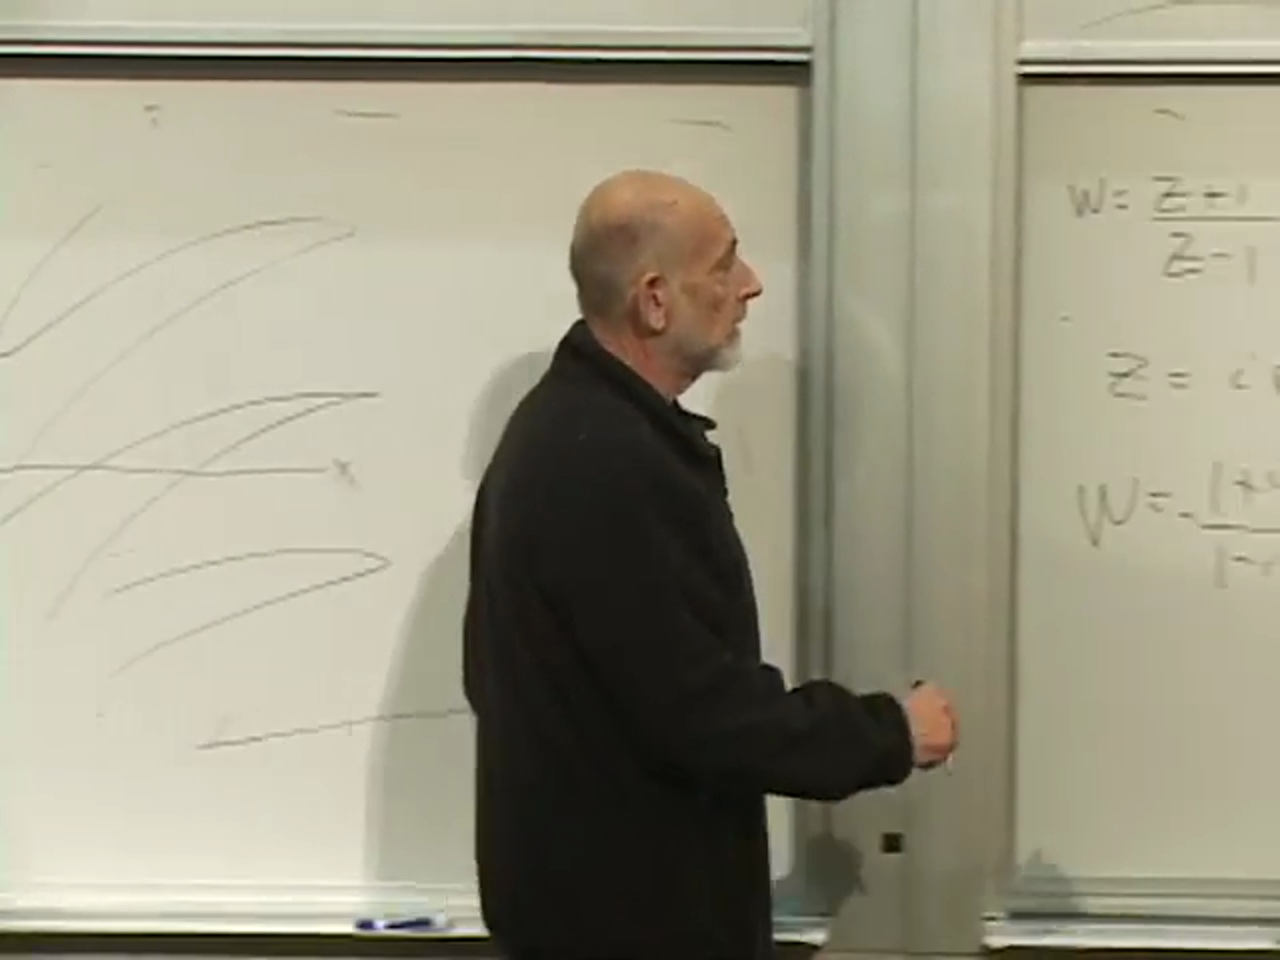
\includegraphics[width=0.72\textwidth]{lecture_08_figure_10.png}
  \caption{单位圆边界的线性分式构造。黑板上可见的倒数约定交换了内部与外部。}
  \lectureframe{00:58:38}
  \label{fig:l08-cayley-board}
\end{figure}

Möbius映射将圆和直线的广义集合映为圆和直线。因此，半平面上的径向和圆周网格在圆盘上变成两族正交的弧。直线直径不过是圆心趋于无穷远的圆的极限情形。

\begin{classroomqa}
\audiencequestion{在圆盘内部画出的弧真的是圆吗？\lecturetimestamp{01:00:55}}
\lecturerresponse{是的。它们的圆心位于不同位置，常常在可见圆盘之外。直径是同一族中半径趋于无穷的极限。}
\end{classroomqa}

\begin{classroomqa}
\audiencequestion{圆盘的图是否意味着它是一个球面，另一个半平面到哪里去了？\lecturetimestamp{01:01:21}}
\lecturerresponse{这里的图是一个平直的圆盘，不是球面。右半平面映到其边界内部，左半平面映到外部。如果向整个复平面添加无穷远点，那么该扩充平面可以通过球极投影表示为球面；那是一个不同的整体陈述。}
\end{classroomqa}

\begin{classroomqa}
\audiencequestion{哪些圆盘曲线对应于原来的径向辐条和固定半径的半圆？\lecturetimestamp{01:02:59}}
\lecturerresponse{正实轴变成连接\(-1\)和\(+1\)的直径。其他射线变成连接同样这些边界点的圆弧。固定半径的半圆变成在单位圆上开始并结束的正交族。}
\end{classroomqa}

\begin{figure}[H]
  \centering
  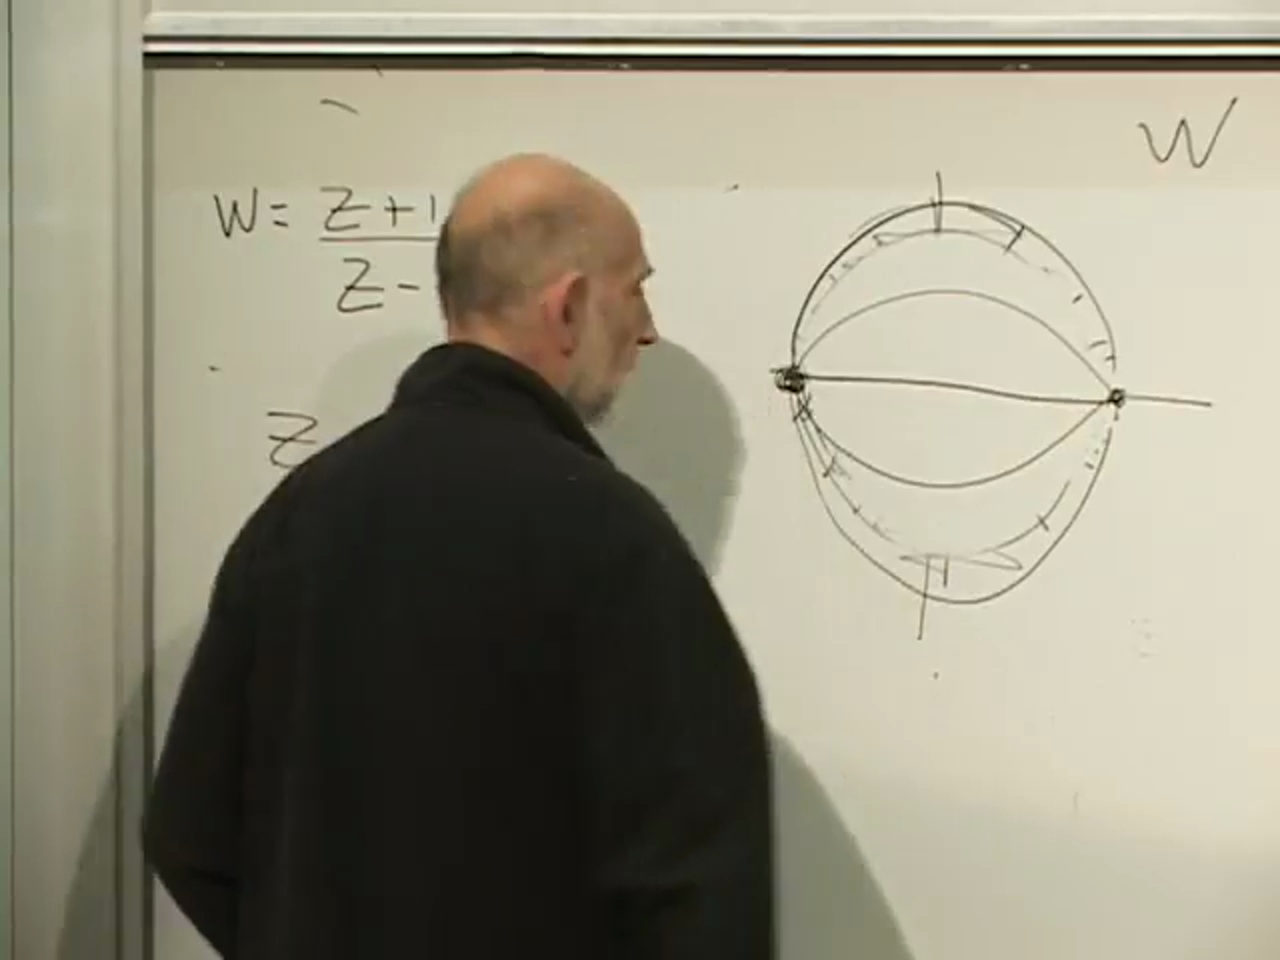
\includegraphics[width=0.72\textwidth]{lecture_08_figure_11.png}
  \caption{半平面中的直线和半圆变成圆盘中的正交圆与直线族。}
  \lectureframe{01:03:48}
  \label{fig:l08-circle-grid-board}
\end{figure}

\section{四弦世界面}

现在我们可以回到散射。两条开弦进入，结合成一条弦，传播任意一段时间，然后分裂成两条出射弦。在带子坐标中，世界面看起来像一条长带子，从两端各有一条缝---这就是“运动绷带”图像。中间寿命不是预先选定的。它是振幅所积分的诸多历史之一。

设\((\sigma,\tau)\)为世界面上的坐标，并设
\begin{equation}
  X^\mu=X^\mu(\sigma,\tau)
  \label{eq:l08-embedding}
\end{equation}
给出它在时空中的位置。标签\(\sigma,\tau\)位于二维参数曲面上；指标\(\mu\)标记时空坐标。在玻色弦理论中\(\mu=0,\ldots,25\)；在超弦情形中有十个时空坐标。

经过 Wick 转动后，自由嵌入场具有欧几里得作用量
\begin{equation}
  S_E[X]
  =\frac{1}{4\pi\alpha'}\int_\Sigma d\sigma\,d\tau\,
  \left[
    \partial_\tau X^\mu\partial_\tau X_\mu
    +\partial_\sigma X^\mu\partial_\sigma X_\mu
  \right].
  \label{eq:l08-euclidean-action}
\end{equation}
相应的路径积分对所选世界面到时空的每一个嵌入求和：
\begin{equation}
  \int\mathcal D X\,e^{-S_E[X]}.
  \label{eq:l08-bare-worldsheet-integral}
\end{equation}

\begin{figure}[H]
  \centering
  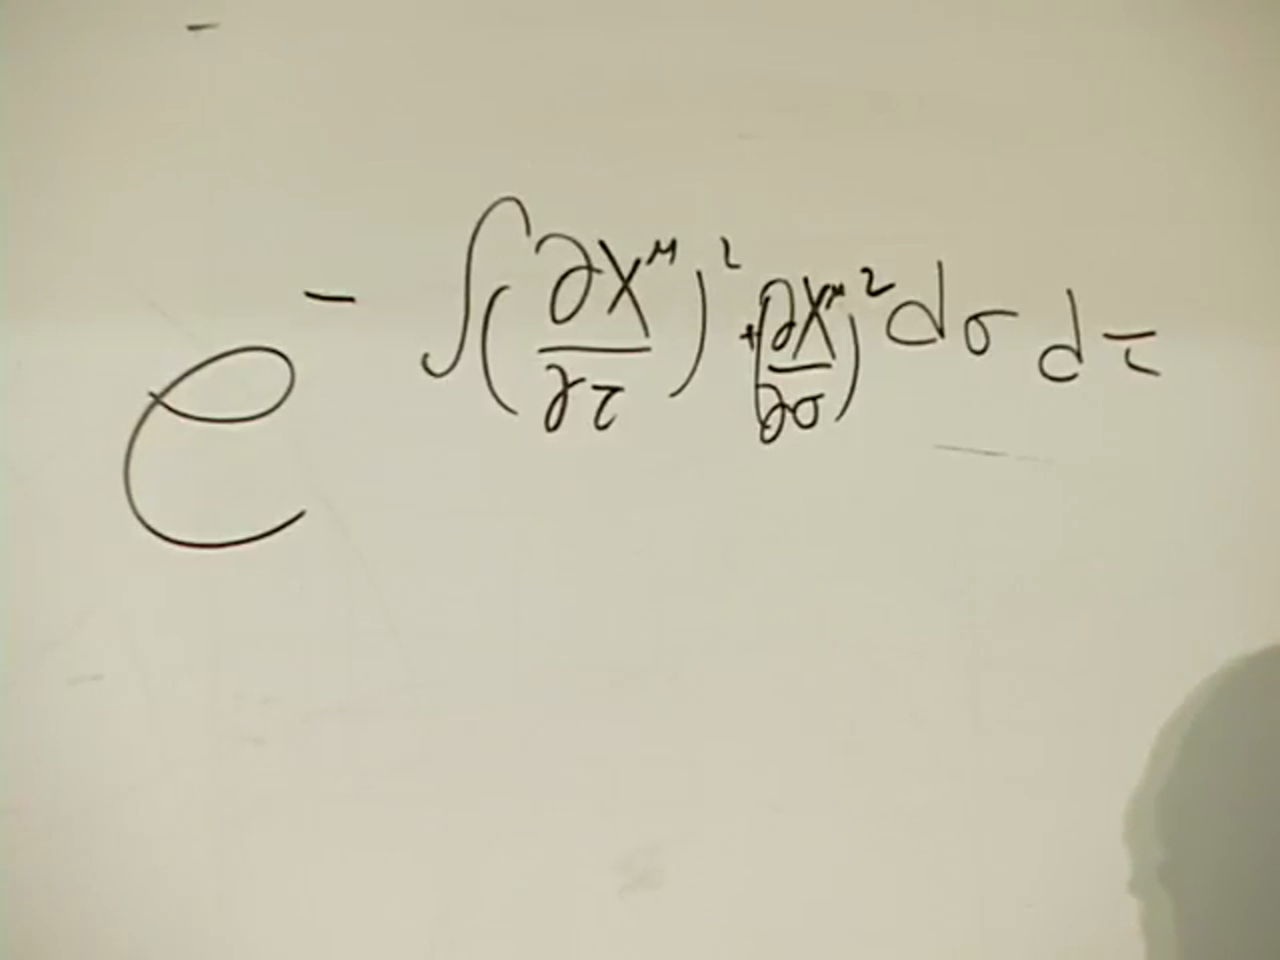
\includegraphics[width=0.74\textwidth]{lecture_08_figure_12.png}
  \caption{完整的正欧几里得世界面权重。两个导数项对所有时空分量求和。}
  \lectureframe{01:11:34}
  \label{fig:l08-action-board}
\end{figure}

带缝长条只有一个连通边界。因此，共形自由度允许将它表示为一个圆盘。长条的四个远端成为边界上的四个标记点。形变这些标记点会改变长条坐标中连接与分裂之间的表观间隔，但不会改变底层的曲面或物理。

\begin{figure}[H]
  \centering
  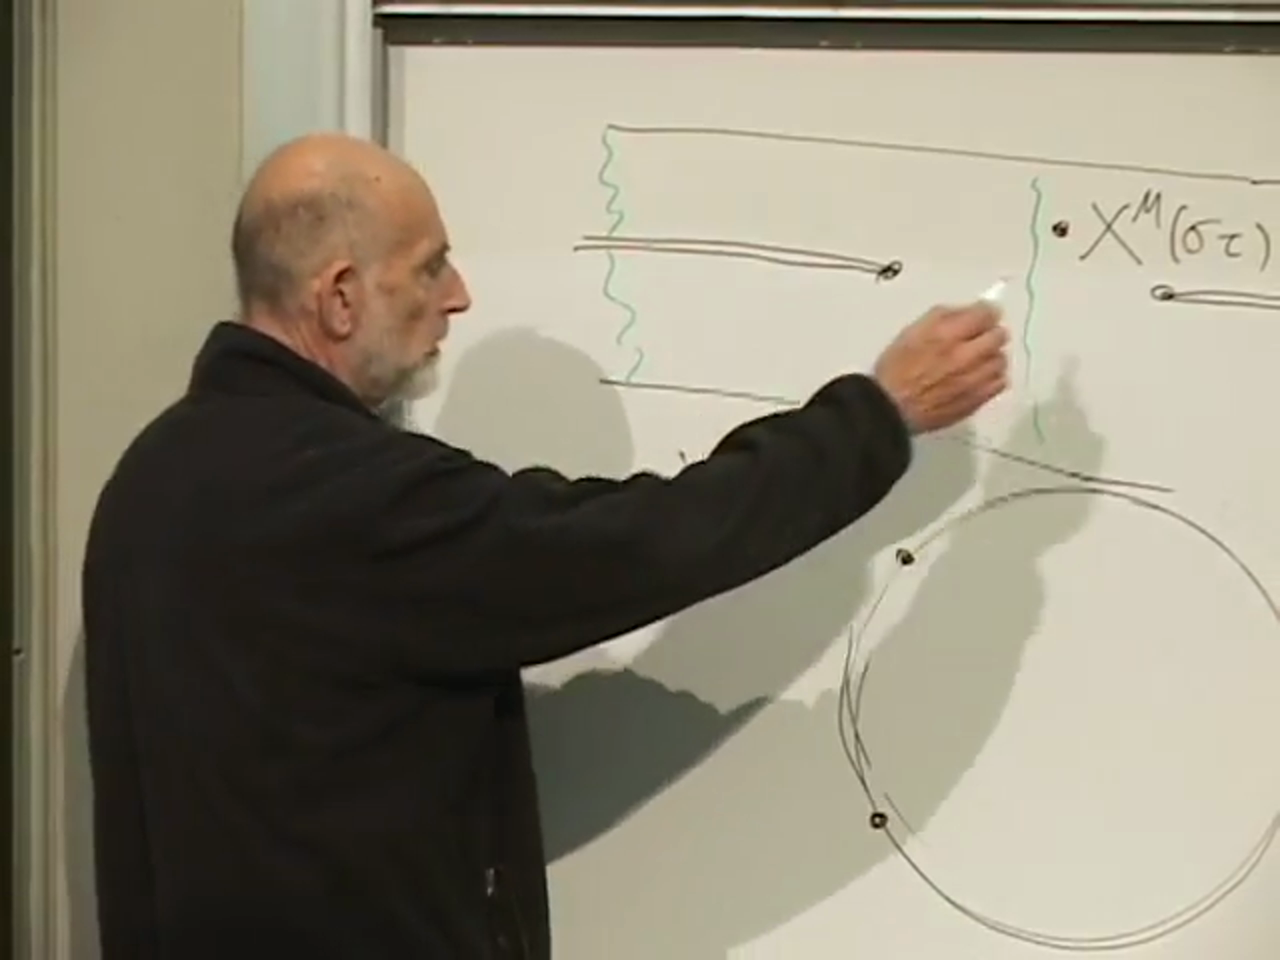
\includegraphics[width=0.76\textwidth]{lecture_08_figure_13.png}
  \caption{带缝长条世界面及其圆盘表示，边界点对应外部弦。}
  \lectureframe{01:15:18}
  \label{fig:l08-bandage-disc-board}
\end{figure}

用来描绘这个共形映射的详细网格线不携带任何物理内容。重要的是拓扑、边界以及标记的外部点。同一个世界面可以被拉伸成不同的通道图像，而不会引入新的相互作用。

\section{外部态作为边界插入}

裸积分 \eqref{eq:l08-bare-worldsheet-integral} 尚未说明哪些动量进入、哪些动量离开。对于动量为 \(k_i^\mu\) 的标量开弦态，在边界上插入顶点算符
\begin{equation}
  V_i(z_i)=e^{\,i k_i\cdot X(z_i)},
  \qquad
  k_i\cdot X=k_{i\mu}X^\mu.
  \label{eq:l08-vertex}
\end{equation}
点 \(z_i\) 是世界面边界上的一个位置。它不是时空坐标，也不是动量的方向。

\begin{figure}[H]
  \centering
  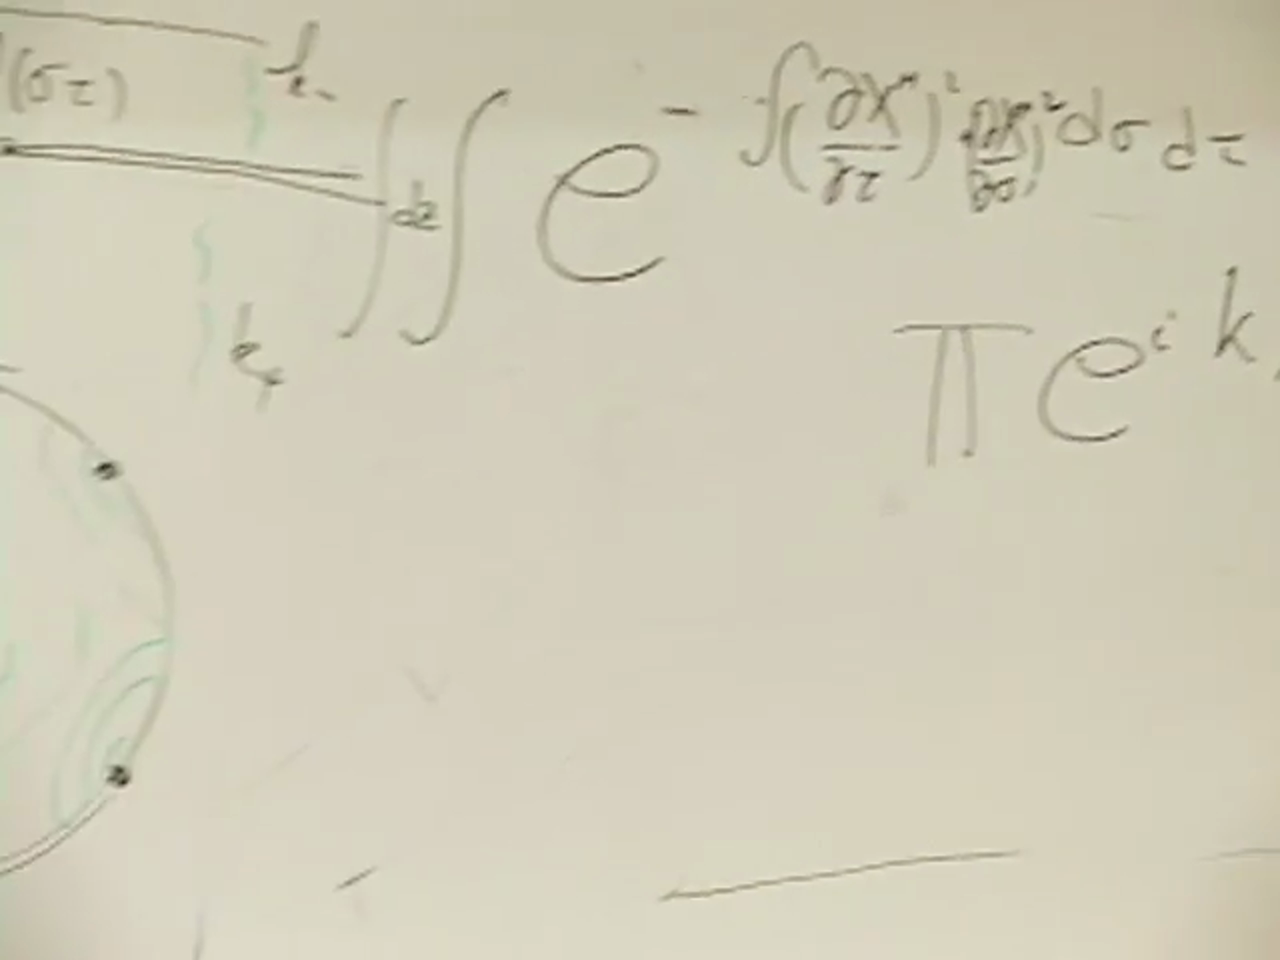
\includegraphics[width=0.72\textwidth]{lecture_08_figure_14.png}
  \caption{体欧几里得权重与边界动量插入的乘积被显示为不同的因子。}
  \lectureframe{01:18:58}
  \label{fig:l08-vertex-board}
\end{figure}

对于 \(n\) 条外部开弦，示意性的规定是
\begin{equation}
  \begin{aligned}
    \mathcal A_n(k_1,\ldots,k_n)
    &=\int_{\mathcal M_{0,n}^{\partial}}\!d\mu(z_i)
      \int\mathcal D X\\
    &\quad\times e^{-S_E[X]}
      \prod_{i=1}^{n}e^{\,i k_i\cdot X(z_i)}.
  \end{aligned}
  \label{eq:l08-open-string-prescription}
\end{equation}
泛函积分是对嵌入 \(X^\mu\) 进行的。有限维积分是对不等价的边界插入位置进行的。极化因子和规范固定测度在此阶段被省略，正如讲座中那样。
\editorialnote{一个完整的规范固定弦振幅还包含相应的鬼场贡献、依赖于态的顶点因子、耦合常数和归一化。方程
\eqref{eq:l08-open-string-prescription} 记录了本讲座中展开的嵌入场依赖和位置依赖。}

\begin{classroomqa}
\audiencequestion{如果外部动量是固定的，为什么还要对它们积分？\lecturetimestamp{01:20:42}}
\lecturerresponse{它们并没有被积分。\(k_i\) 是散射振幅的固定标记。被积分的是嵌入场以及那些固定动量所插入的世界面位置 \(z_i\)。后一个积分取代了长条图像中对中间寿命的积分。}
\end{classroomqa}

\begin{classroomqa}
\audiencequestion{顶点因子的乘积是在路径积分内部，它是作用量的一部分吗？\lecturetimestamp{01:21:39}}
\lecturerresponse{它是在泛函积分内部乘在 \(e^{-S_E}\) 上。也可以等价地将这些因子指数化，并把它们视为加到作用量上的局域源项，但它们在概念上是顶点算符，而不是自由体作用量的一部分。}
\end{classroomqa}

\begin{figure}[H]
  \centering
  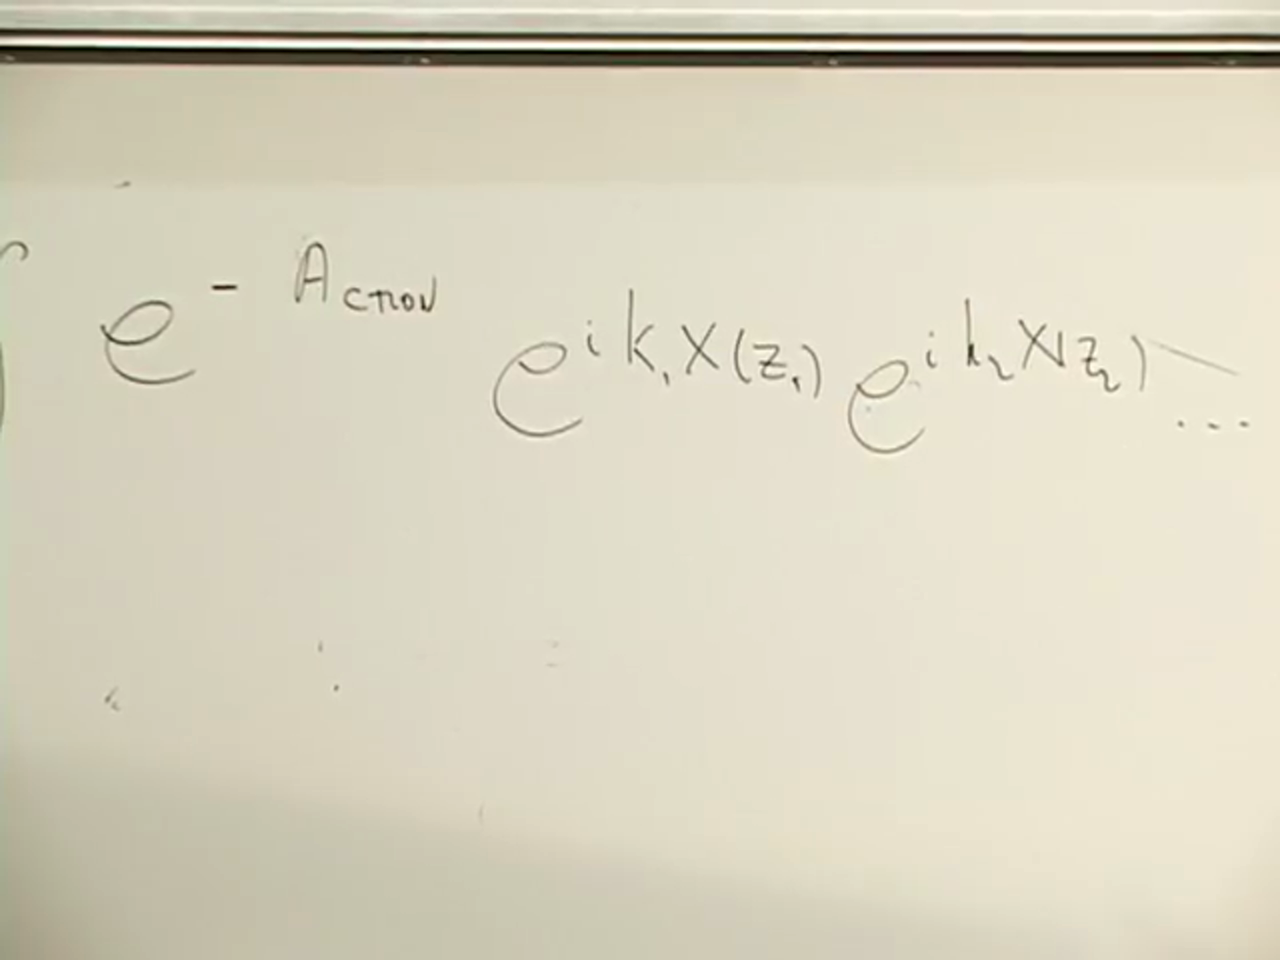
\includegraphics[width=0.76\textwidth]{lecture_08_figure_15.png}
  \caption{用分离的因子 \(e^{ik_i\cdot X(z_i)}\) 表示相继外部粒子的路径积分。}
  \lectureframe{01:23:23}
  \label{fig:l08-full-prescription-board}
\end{figure}

\begin{classroomqa}
\audiencequestion{为什么在世界面 Wick 转动之后 \(e^{ik\cdot X}\) 仍然含有 \(i\)？\lecturetimestamp{01:23:42}}
\lecturerresponse{该转动改变了世界面时间，并将体权重从 \(e^{iS}\) 转换为 \(e^{-S_E}\)。动量本征函数中的 \(i\) 是标记时空动量的傅里叶相位。它起着不同的作用，并且保留下来。}
\end{classroomqa}

\begin{classroomqa}
\audiencequestion{位置 \(z_i\) 是否决定动量矢量的方向？\lecturetimestamp{01:24:19}}
\lecturerresponse{不决定。方向编码在时空分量 \(k_i^\mu\) 中。插入点 \(z_i\) 说明该动量从何处进入世界面描述；\(X^\mu(z_i)\) 是 \(\mathcal D X\) 所求和的对象之一。}
\end{classroomqa}

\begin{classroomqa}
\audiencequestion{所画的绷带腿的角度是否编码了物理动量的方向？\lecturetimestamp{01:25:07}}
\lecturerresponse{不编码。绷带是参数空间，不是弦在物理时空中的图像。它的腿可以画成水平的、倾斜的或共形弯曲的。物理方向由分量 \(k^\mu\) 承载，而 \(X^\mu(\sigma,\tau)\) 则被积分掉。}
\end{classroomqa}

\section{作为静电学的高斯积分}

作用量\eqref{eq:l08-euclidean-action}对每个分量\(X^\mu\)都是二次的，而一旦把插入算符的指数与作用量合并，这些插入就表现为线性源。因此泛函积分是高斯型的。在其鞍点处，每个时空分量都满足一个示意形式为
\begin{equation}
  \nabla^2 X^\mu(z)
  \propto
  i\alpha'\sum_i k_i^\mu\,\delta(z-z_i),
  \label{eq:l08-electrostatic-source}
\end{equation}
的泊松方程，并带有圆盘边缘上的开弦边界条件。每个\(X^\mu\)的行为都像一个独立的静电势，而每个动量分量\(k_i^\mu\)的行为则像置于\(z_i\)处的相应电荷。

\begin{figure}[H]
  \centering
  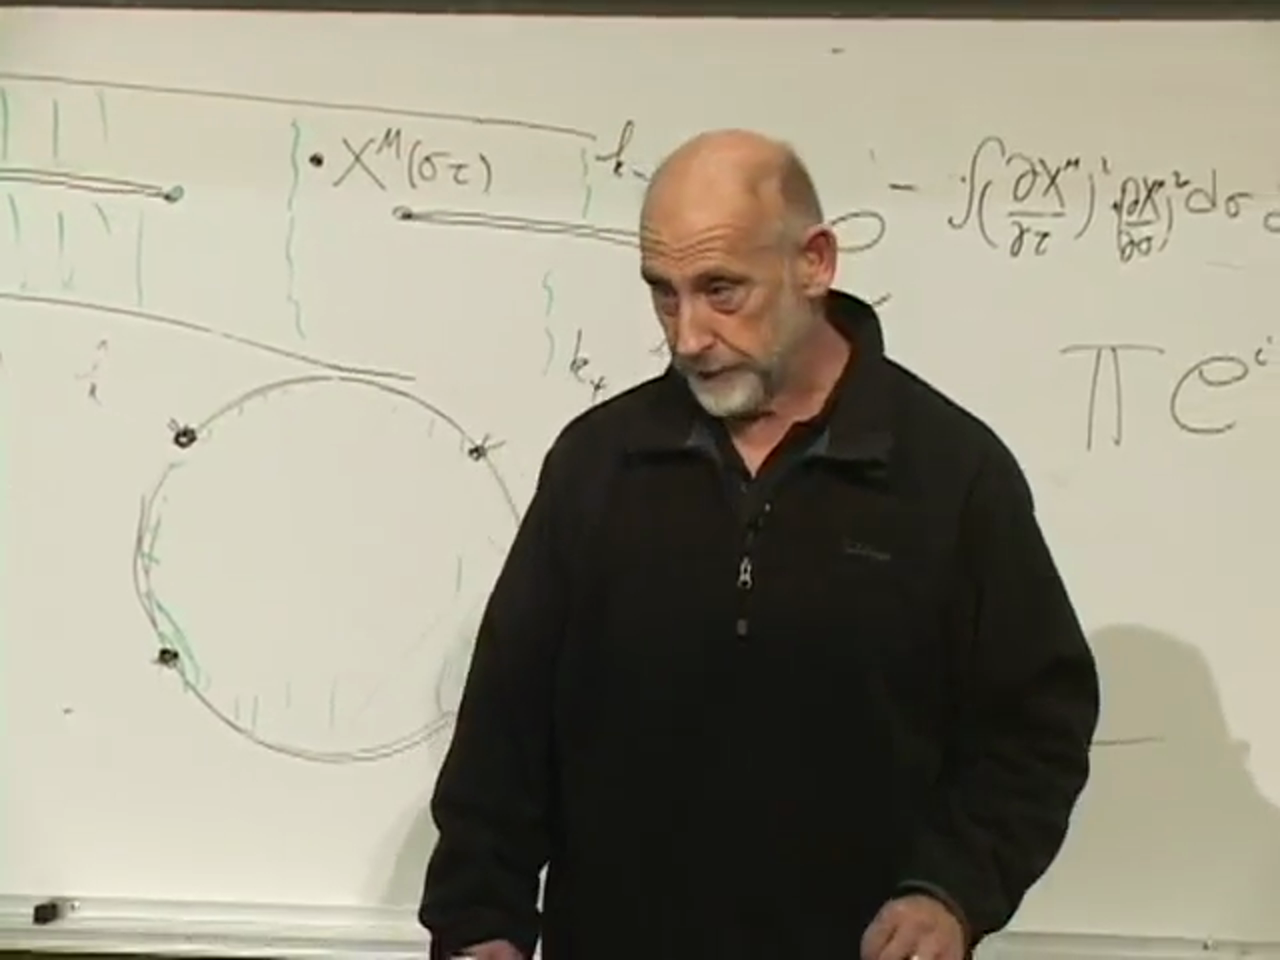
\includegraphics[width=0.76\textwidth]{lecture_08_figure_16.png}
  \caption{带有边界源的圆盘被解释为：对每个时空分量各有一个独立的二维静电场问题。}
  \lectureframe{01:28:58}
  \label{fig:l08-electrostatic-disc-board}
\end{figure}

求解该静电场问题，计算其能量，对负能量取指数，最后对不等价的电荷位置积分。在标准的开弦归一化下，嵌入场关联函数给出 Koba--Nielsen 因子
\begin{equation}
  \left\langle\prod_i e^{\,ik_i\cdot X(z_i)}\right\rangle
  \propto
  (2\pi)^D\delta^{(D)}\!\left(\sum_i k_i\right)
  \prod_{i<j}|z_i-z_j|^{2\alpha' k_i\cdot k_j}.
  \label{eq:l08-koba-nielsen}
\end{equation}
该 delta 函数表示动量守恒。乘积中包含静电场成对能量。对于此处所用的四个标量边界插入，固定三个位置后，剩余积分就化为前几讲中遇到的 Euler beta 积分。

\begin{classroomqa}
\audiencequestion{是有二十六个静电能，还是只有一个？
\lecturetimestamp{01:30:53}}
\lecturerresponse{对每个时空分量，都有一个独立的势和场。在一个正交归一的靶空间基中，它们的二次能量没有交叉项，并且这些贡献在取指数之前被加到一个总作用量中。}
\end{classroomqa}

\begin{classroomqa}
\audiencequestion{圆盘的角坐标就是物理散射角吗？\lecturetimestamp{01:32:10}}
\lecturerresponse{不是。它是一个世界面位置参数。它的不等价组合与中间传播间隔有关，并且要被积分掉。物理散射角通过由固定动量构造的 Lorentz 不变量来编码。}
\end{classroomqa}

\begin{classroomqa}
\audiencequestion{为什么这一构造在临界维数之外会失效？
\lecturetimestamp{01:32:35}}
\lecturerresponse{仅靠形式上的高斯积分并不是全部一致性条件。规范固定会引入一个共形反常，其物质贡献与鬼场贡献只有在临界维数下才会相消：玻色弦为\(D=26\)，超弦为\(D=10\)。若没有这种相消，量子世界面所假定的共形对称性就会丧失。}
\end{classroomqa}

\begin{classroomqa}
\audiencequestion{我们是否已经假定了三个大的空间维和紧致额外维？\lecturetimestamp{01:33:38}}
\lecturerresponse{没有。紧致化尚未进入这一构造。在这个阶段，玻色坐标仍然取遍全部二十六个靶空间方向，或者在超弦情形下取遍十个方向。一个子集如何能够保持宏观上很大，是下一次讨论的主题。}
\end{classroomqa}

\begin{classroomqa}
\audiencequestion{与静电学的联系仅仅在于坐标满足 Laplace 方程吗？\lecturetimestamp{01:33:57}}
\lecturerresponse{正是如此。在插入点之外，每个\(X^\mu\)都是调和的；顶点算符提供 delta 函数源。无论我们是否使用静电学的词汇，这在数学上都是与带点电荷的静态二维势相同的边值问题。}
\end{classroomqa}

\subsection{共形冗余与模的数目}

圆盘具有一个三实参数的共形自同构群，\(\mathrm{PSL}(2,\mathbb R)\)。因此，三个有序边界点可以被固定在方便的位置上。对于四个外弦，只剩下第四个位置需要积分；对于\(n\)个有序边界插入，树图阶有
\begin{equation}
  n-3
  \label{eq:l08-n-minus-three}
\end{equation}
个实位置积分。

\begin{classroomqa}
\audiencequestion{圆盘周围有四个独立的角位置吗？\lecturetimestamp{01:34:37}}
\lecturerresponse{物理上没有。起初写出四个位置，但圆盘的共形对称性可以把任意三个放到方便之处。对于两进两出振幅，只剩下第四个的相对位置需要处理。}
\end{classroomqa}

\begin{figure}[H]
  \centering
  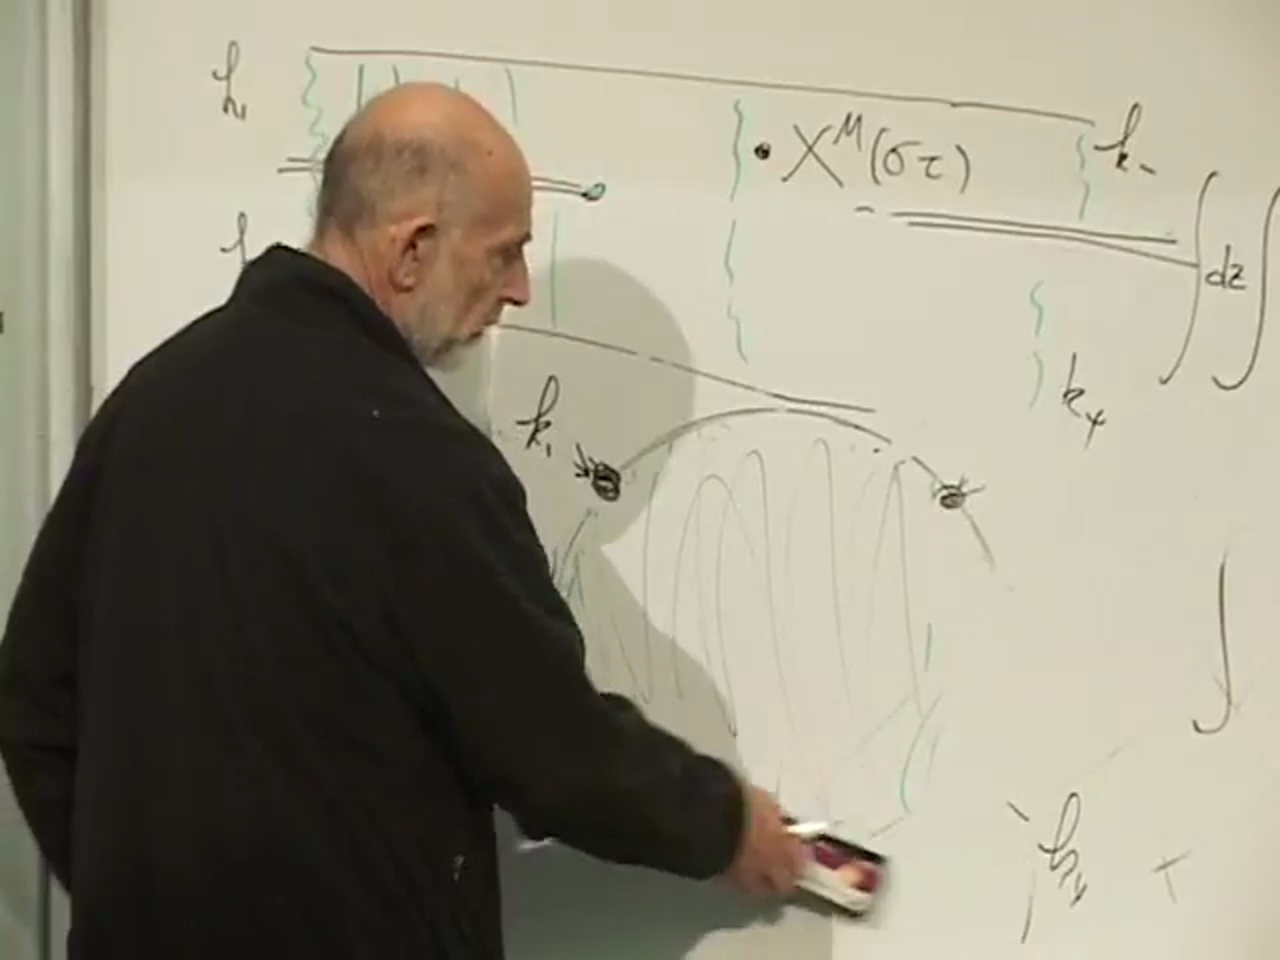
\includegraphics[width=0.72\textwidth]{lecture_08_figure_17.png}
  \caption{圆盘上的四个边界插入。共形自由度固定任意三个，留下一个四点模。}
  \lectureframe{01:35:18}
  \label{fig:l08-fix-three-board}
\end{figure}

\begin{classroomqa}
\audiencequestion{如果条带图中两个分裂点不在同一高度，会怎样？\lecturetimestamp{01:35:24}}
\lecturerresponse{共形映射可以把这种表观不匹配移走。不同的图是同一个模的不同坐标代表。不变的积分是对剩余边界位置的积分，等价地，也就是对传播间隔的积分。}
\end{classroomqa}

\begin{classroomqa}
\audiencequestion{对于更多的外部粒子，还剩下多少个位置参数？\lecturetimestamp{01:36:00}}
\lecturerresponse{利用共形对称性固定三个插入点，并对另外\(n-3\)个进行积分。这就是有序树级开弦振幅的边界模数计数。}
\end{classroomqa}

\begin{classroomqa}
\audiencequestion{这与M理论有何关系？\lecturetimestamp{01:36:37}}
\lecturerresponse{目前还没有。这里的构造是世界面上的微扰开弦散射。它与M理论的关系需要后来的对偶性和非微扰思想，因此这个问题被明确推迟。}
\end{classroomqa}

\begin{classroomqa}
\audiencequestion{不同的竖直或交叉条形图景是否是不同的计算？\lecturetimestamp{01:36:49}}
\lecturerresponse{不是。可以固定一个方便的点，并让其余的模数在其整个区间内变化。条形图景和圆盘上的边界点积分是同一个积分的不同切片方式，这就是为什么所有外部弦都可以被对称地处理。}
\end{classroomqa}

\section{该方案尚未解决的问题}

圆盘公式可以直接推广到更多外部弦：加入更多顶点算符，并对它们的\(n-3\)个不等价边界位置进行积分。对于一个自洽的弦模型来说，这是一个精确的树级方案，但它还不是一个关于已观测粒子物理的现实模型。简单的玻色子理论具有错误的时空维数和额外的物理缺陷。超弦改进了谱，并将临界维数降低到十，但仍然必须紧致化六个空间维度。

\begin{classroomqa}
\audiencequestion{这个简单模型是否已经与粒子碰撞实验一致？\lecturetimestamp{01:39:06}}
\lecturerresponse{不一致。其共振结构在历史上类似于强子散射，但二十六维玻色子模型不能直接描述已观测到的粒子。该形式体系为模型定义了散射振幅；要与自然相符，还需要现实的谱、紧致化、相互作用以及真空选择。}
\end{classroomqa}

\begin{classroomqa}
\audiencequestion{紧致化会减少额外维度并产生现实的粒子数据吗？\lecturetimestamp{01:41:10}}
\lecturerresponse{它可以降低有效宏观维度，并生成粒子谱和规范群。真正的数学困难也大多出现在这里。人们已经知道许多自洽的紧致化，但选择一个关于已观测基本粒子的唯一模型仍未解决。}
\end{classroomqa}

本讲强调这一区分，而不是宣传一个已经完成的理论。弦构造在数学上是确定的，并且已经产生了关于引力和几何的深刻信息，然而它们的多重性本身就是物理问题的一部分。

\begin{classroomqa}
\audiencequestion{有没有一种简短的方法来记住为什么玻色子临界维数是二十六？\lecturetimestamp{01:43:19}}
\lecturerresponse{先前的振子计算使用了正则化的零点求和\(1+2+3+\cdots=-1/12\)。横向振子贡献涉及二十四个方向，而恢复两个纵向时空坐标后得到\(24+2=26\)。这是对先前一致性论证的记忆法，而不是这里的新推导。}
\end{classroomqa}

\begin{classroomqa}
\audiencequestion{插入的动量\(k_i\)本身是量子化的吗？\lecturetimestamp{01:43:46}}
\lecturerresponse{在非紧致时空中，其分量是连续的。被量子化的是振子能级，从而是允许的质量平方谱。紧致维度可能会量子化相应的动量和绕数分量，但那属于下一次讨论。}
\end{classroomqa}
